% !TEX root = ../../技术文档.tex
\section{模型部署与应用软件}

\subsection{模型选型}

系统采用YuNet人脸检测网络\cite{wu2023yunet}，以OpenCV Zoo发布的\path{face_detection_yunet_2023mar.onnx}为权重来源\cite{opencv-zoo-yunet-2023mar}。
YuNet采用无锚框检测结构，由特征提取主干、轻量特征金字塔（TFPN）和检测头组成，原始网络结构如图\ref{fig:yunet-architecture}所示。
主干利用逐点卷积与深度卷积提取图像特征，TFPN通过上采样和逐元素相加融合不同尺度的特征，检测头据此预测不同尺寸的人脸。
逐点卷积和深度卷积分别映射到NPU的通道归约与通道独立计算通路，固定输入尺寸便于离线确定各层形状及存储布局。

\begin{figure}[!htbp]
    \centering
    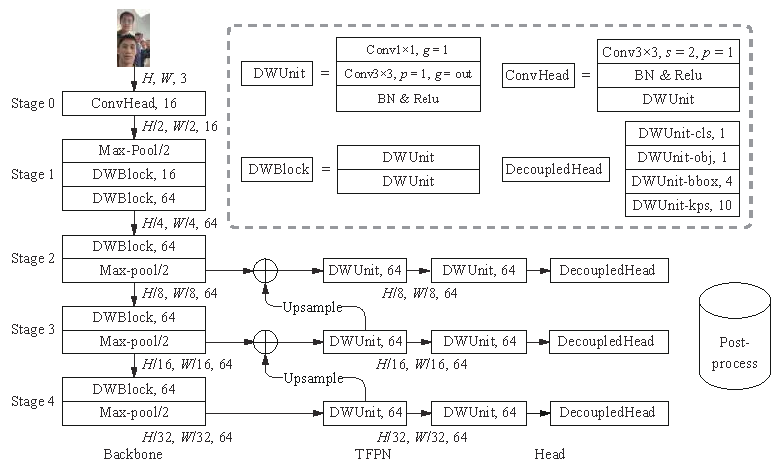
\includegraphics[width=\linewidth]{../figure/yunet-paper-architecture.pdf}
    \caption[YuNet原始网络结构]{YuNet原始网络结构（引自文献\cite{wu2023yunet}图4，\href{https://creativecommons.org/licenses/by/4.0/}{CC BY 4.0}）}
    \label{fig:yunet-architecture}
\end{figure}

本项目部署图将输入固定为$[1,3,320,320]$，裁剪原图中的关键点预测（kps）及其依赖分支，保留分类概率cls、目标概率obj和检测框bbox输出，保留分支的权重不变。
步长为8、16、32的三个检测尺度分别对应40$\times$40、20$\times$20和10$\times$10的网格，每个尺度输出cls、obj和bbox，共九组输出。
对于板级800$\times$600输入，Video将图像缩放为320$\times$240，上下各补40行零值，形成320$\times$320模型输入。
NPU完成定点网络计算，CPU对九组输出进行解码和非极大值抑制（NMS），选择主人脸并提交显示记录，Video在同帧原图上绘制检测框或合成透明头像。

部署包记录权重来源、版本和哈希，以及固定形状计算图的算子、张量和输出顺序。
输入尺寸、预处理、量化和后处理参数作为同一配置管理，浮点与整数参考采用相同的输入画面和候选筛选规则。

\subsection{量化方案}

外部输入采用UINT8 BGR NCHW，保留0至255像素值，尺度为1、零点为0。
首层直接以U8激活乘S8权重，不进行减128转换。网络内部按张量选择U8或S8：融合ReLU的输出为U8，非ReLU的8位输出为S8。
权重采用$[-127,127]$的对称INT8编码和逐输出通道尺度，激活采用逐张量尺度\cite{krishnamoorthi2018quantization}，全部零点为0。
Bias按输入尺度与权重尺度的乘积量化为INT32，完整卷积和加Bias后仅重定标一次；系数乘法保留64位精度，最近偶数舍入后按输出范围饱和。
BN融合、重定标系数及移位在线下生成，Add以共同移位分母对两路输入尺度对齐后相加，只进行一次舍入和饱和。

表\ref{tab:npu-stage-types}列出卷积主干与检测框、概率输出的类型。表中S8、S16使用对称范围$[-127,127]$、$[-32767,32767]$；
U8和U16分别覆盖$[0,255]$、$[0,65535]$，激活的符号属性随算子记录切换，零点列按激活/权重顺序列出。

\begin{reporttable}
\begin{longtable}{@{}p{0.20\linewidth}p{0.10\linewidth}p{0.09\linewidth}p{0.12\linewidth}p{0.18\linewidth}p{0.14\linewidth}@{}}
\caption{NPU各阶段整数类型}\label{tab:npu-stage-types}\\
\toprule
阶段 & 激活 & 权重 & 零点 & 累加类型 & 输出 \\
\midrule
\endfirsthead
\caption[]{NPU各阶段整数类型（续）}\\
\toprule
阶段 & 激活 & 权重 & 零点 & 累加类型 & 输出 \\
\midrule
\endhead
\bottomrule
\endfoot
视频输入与补边 & U8 & --- & 0/--- & --- & U8 \\
首层3$\times$3卷积 & U8 & S8 & 0/0 & S24本地和，扩展至INT32 & U8（ReLU） \\
后续普通/逐点卷积 & U8或S8 & S8 & 0/0 & S24本地和，扩展至INT32 & S8 \\
深度卷积 & S8 & S8 & 0/0 & INT32 & U8或S16 \\
概率Sigmoid & S8 & --- & 0/--- & 索引重定标、查表 & U16 \\
\end{longtable}
\end{reporttable}

首层U8输出经后续逐点卷积重定标为S8，再进入S8$\times$S8深度卷积。
视频上下补边与卷积窗口越界补边均写入整数0，表示实数0；没有输入偏移引入的Bias补偿项。

离线工具以代表性图像进行训练后量化（PTQ）校准\cite{krishnamoorthi2018quantization}，记录逐层浮点与整数误差，硬件按整数参考中的舍入及饱和规则执行。
板级800$\times$600输入采用固定5:2双线性缩放，按BGR顺序组织，并在上下各补40行零值。
WIDER校准与验证按各图像的原始长宽比，将长边缩放至320像素，短边尺寸按就近取整、半数取偶规则确定，再居中补零至320$\times$320；奇数余量置于右侧或下侧。
FP32与软件整数参考共用该数据集预处理流程。
输入不附加除以255的归一化，也不补齐至八个通道。

PTQ从WIDER FACE训练集中选取512张与验证集无内容重复的图像进行校准，在全部3226张验证图像上比较FP32与bbox16软件整数参考。
bbox16保留INT16框回归输出，概率采用U16 Q0.16，其余卷积激活按U8/S8编码。
AP评价采用候选分数阈值0.001、NMS IoU阈值0.3及5000的候选上限，按官方难度子集以IoU不小于0.5匹配，计算1000个阈值的VOC AP；0.6用于单独的工作点分析。结果如下表所示。

\begin{reporttable}
\begin{longtable}{@{}lrrr@{}}
\caption{YuNet软件整数参考的检测精度}\\
\toprule
难度 & FP32 AP（\%） & bbox16 AP（\%） & AP下降（百分点） \\
\midrule
\endfirsthead
\caption[]{YuNet软件整数参考的检测精度（续）}\\
\toprule
难度 & FP32 AP（\%） & bbox16 AP（\%） & AP下降（百分点） \\
\midrule
\endhead
\bottomrule
\endfoot
Easy & 78.3929 & 78.2039 & 0.1889 \\
Medium & 67.2333 & 66.9742 & 0.2591 \\
Hard & 31.5613 & 31.3584 & 0.2029 \\
\end{longtable}
\end{reporttable}

AP下降按未舍入原值计算，各项分别保留四位小数。Easy差值0.188946个百分点舍入后为0.1889。
在本项目固定320单尺度预处理及相同后处理、评价规则下，bbox16相对FP32的AP最大下降为0.2591个百分点，整数方案的增量损失较小。
当前FP32基线的Hard AP为31.5613\%，固定320输入下的小脸检测仍受限制。
OpenCV Zoo参考评价按原图尺寸设置输入，候选筛选和结果处理也与本项目不同，因此本表不与官方公布AP直接比较\cite{opencv-zoo-yunet-2023mar}。
本表使用主机端解码及NMS，评价对象为软件整数参考；融合固件定点后处理和板级视频链路的端到端AP需另行评测。

\subsection{模型导出}

导出流程生成固定形状算子表、权重、Bias、量化参数、查找表及张量工作区布局。
逐层记录输入输出形状、有效与存储通道、核尺寸、步长、补边、分组、搬运字节数和生命周期。
模型输入使用B、G、R三平面NCHW布局，中间张量的物理布局、对齐和步长由算子表逐项指定。

部署程序采用NPM3格式，128\,B程序头后依次保存79条128\,B算子记录，总长10,240\,B。
记录给出算子类型、形状、张量引用和数值参数，头部保存模型身份、区域尺寸及校验信息。
模型包包含版本、哈希、预处理配置、输出格式和逐层参考向量。硬件装载器完成各段CRC校验与写入确认后封存模型，CPU提交绑定输入、输出及工作区的整帧任务。
NPU计算图执行器读取程序，解析算子和相对张量引用，并按本帧绑定关系生成层任务。
算子表还记录每层的输入输出区域；跨层连接所需的原张量保留至最后一个使用该张量的算子执行完成。
计算图推进、层内遍历与数据搬运均由NPU完成，模型程序及参数在运行期间保持不变。
CPU解码表独立存放于共享DDR，由软件在检测后处理时按候选读取。

\subsection{算子映射}

普通与逐点卷积使用输入通道归约模式，深度卷积使用通道独立模式；池化、Add和上采样由NPU辅助单元执行。
NPU辅助通路完成概率Sigmoid查表，CPU处理输出候选、框解码和NMS，Video承担输入逐像素处理及显示合成。
部署程序包含30条普通/逐点卷积、17条深度卷积和32条辅助算子记录，共79条；普通/逐点卷积中23条为1$\times$1、7条为3$\times$3。
算子执行方式如下表所列，完整特征图运算均在NPU中完成。

\begin{reporttable}
\setlength{\tabcolsep}{3pt}
\begin{longtable}{@{}p{0.19\linewidth}p{0.06\linewidth}p{0.12\linewidth}p{0.28\linewidth}p{0.27\linewidth}@{}}
\caption{算子执行方式表}\\
\toprule
算子或阶段 & 数量 & 执行单元 & 执行方式 & 数值约定 \\
\midrule
\endfirsthead
\caption[]{算子执行方式表（续）}\\
\toprule
算子或阶段 & 数量 & 执行单元 & 执行方式 & 数值约定 \\
\midrule
\endhead
\bottomrule
\endfoot
普通/逐点卷积 & 30 & NPU & 空间块、16输出通道块，完整$K$归约 & U8/S8乘S8，INT32累加结果 \\
深度卷积 & 17 & NPU & 16通道并行、3$\times$3逐通道计算 & 各通道INT32部分和独立 \\
Add & 2 & NPU & 两源读取、共享量化、向量写回 & 尺度对齐后统一舍入和饱和 \\
MaxPool & 4 & NPU & 2$\times$2、步长2、无补边 & 尺寸向下取整，保持原编码 \\
Resize & 2 & NPU & 最近邻2倍上采样 & 非对称坐标映射、向下取整 \\
Transpose & 9 & NPU & 按固定维序读写 & 保持元素编码 \\
Reshape & 9 & NPU & 按地址和长度搬运 & 保持元素编码与序列 \\
概率Sigmoid & 6 & NPU & 索引重定标、定点查表 & U16，尺度$2^{-16}$ \\
Bias、重定标、激活 & --- & NPU & 融合在卷积记录中 & U8/S8/S16输出，显式饱和 \\
解码、NMS & --- & CPU & 候选筛选、定点查表与排序 & 输出尺度统一，检查中间位宽 \\
缩放、输入格式化 & --- & Video & 流式逐像素处理 & UINT8 BGR NCHW、上下补零 \\
图像叠加 & --- & Video & 原图读取、边框绘制及头像透明合成 & RGB888背景、RGBA8888纹理 \\
\end{longtable}
\end{reporttable}

\subsection{检测后处理}

YuNet部署图按stride 8、16、32输出cls、obj和bbox，320$\times$320输入对应1600、400和100个位置，共2100个预测位置。
每位置包含1个分类概率、1个目标概率和4个框参数，最终均以16位格式交接，有效数据量为$2100\times6\times2=25,200$\,B。
各输出头按部署清单分配跨度，合计26,368\,B；下表偏移均相对于本帧输出槽基址，数据采用小端格式。

\begin{reporttable}
\setlength{\tabcolsep}{5pt}
\begin{longtable}{@{}llrrr@{}}
\caption{九个检测头的输出布局}\\
\toprule
输出头 & 编码 & 字节偏移 & 有效字节 & 分配字节 \\
\midrule
\endfirsthead
\caption[]{九个检测头的输出布局（续）}\\
\toprule
输出头 & 编码 & 字节偏移 & 有效字节 & 分配字节 \\
\midrule
\endhead
\bottomrule
\endfoot
\texttt{cls\_8} & U16 Q0.16 & 0 & 3200 & 3328 \\
\texttt{cls\_16} & U16 Q0.16 & 3328 & 800 & 1024 \\
\texttt{cls\_32} & U16 Q0.16 & 4352 & 200 & 256 \\
\texttt{obj\_8} & U16 Q0.16 & 4608 & 3200 & 3328 \\
\texttt{obj\_16} & U16 Q0.16 & 7936 & 800 & 1024 \\
\texttt{obj\_32} & U16 Q0.16 & 8960 & 200 & 256 \\
\texttt{bbox\_8} & S16 & 9216 & 12800 & 12800 \\
\texttt{bbox\_16} & S16 & 22016 & 3200 & 3328 \\
\texttt{bbox\_32} & S16 & 25344 & 800 & 1024 \\
合计 & --- & --- & 25200 & 26368 \\
\end{longtable}
\end{reporttable}

CPU对NPU输出的U16概率进行阈值筛选，再对保留候选解码；Sigmoid在NPU中查表。
CPU解码表保存按尺度索引的偏移及尺寸变换值，软件将其FP32编码转换为含16位小数的定点数，使用整数运算恢复检测框。

参考分数为$\sqrt{cls\cdot obj}$，筛选阈值为0.6。概率头采用相同尺度，软件先比较概率乘积与阈值平方对应的整数界限，再为通过筛选的候选生成舍入后的分数。
候选按分数降序、候选序号升序处理，使用64项缓冲分页排序；NMS保留结果跨页累计，直到得到16个有效框或遍历完符合阈值的候选。
贪心NMS在IoU大于0.3时抑制候选，利用$10I>3U$比较交集面积$I$和并集面积$U$，以整数运算实现门限判定。
检测坐标扣除补边后恢复到原始800$\times$600画面：
\[
x_{\mathrm{raw}}=\frac{5}{2}x_{\mathrm{net}},\qquad
y_{\mathrm{raw}}=\frac{5}{2}(y_{\mathrm{net}}-40)
\]
框采用左闭右开范围，坐标扣除补边并裁剪至有效图像区域后按5:2映射到原图，左上角向下取整、右下角向上取整；删除零面积框及补边区无效候选。

主人脸从保留的NMS结果中选择，优先取有效面积最大者，同面积时按分数高者、候选序号小者决定。
CPU将保留框和主人脸索引写入显示记录，并以主框尺寸及素材锚点计算头像覆盖区域。显示模式为RAW、BOX或AVATAR，由按键请求经软件提交；头像定位、缩放与透明合成见第\ref{sec:video-overlay}节。
显示记录中的原图坐标与帧号、槽号及会话身份共同提交，使检测结果与所显示的原图对应。

\subsection{裸机运行时}

配置位流初始化Boot ROM及SRAM中的固件内容，CPU从Boot ROM跳转到\texttt{0x0001\,0000}处的应用入口。
应用代码、只读数据、变量和栈位于32\,KiB SRAM；启动代码设置栈及异常入口、清零BSS，然后进入主循环。
DDR初始化和HDMI器件配置由板级硬件完成，模型及头像素材通过硬件UART装载器在启动阶段写入DDR。

装载顺序为NPM3程序、参数镜像、CPU解码表、A、B、C三个输出槽的头数据初值及RGBA头像。前六段模型数据共1,770,496\,B，头像为262,144\,B，七段合计2,032,640\,B。
UART采用115200\,baud、8N1，装载器按256\,B载荷接收数据包，核对段号、偏移和CRC，并等待DDR写入确认；七段数据均通过校验后封存模型及素材。
仅传输有效载荷的理论时间为$2,032,640\times10/115200\approx176.444$\,s。
计入每包16\,B包头及12\,B确认包后，7,940包的停等协议线速预算约为195.743\,s，尚未计入主机调度、确认周转及DDR等待。
装载记录没有保存实际起止时刻，因此上述数值仅为启动传输预算，与逐帧推理耗时分别统计。
CPU轮询NPU就绪状态，重复读取IDLE与有效会话标识并确认一致，随后初始化三帧槽、选择RAW模式并开放采集和推理。

驱动封装整帧NPU、采集、显示及帧池接口，公共配置生成硬件与软件共用的地址和寄存器定义。
帧记录维护槽号、帧号、会话身份、地址及状态；CPU候选缓冲和显示记录位于SRAM，中间张量及九头输出位于共享DDR。
应用采用轮询主循环，依次处理显示事件、采集完成、NPU完成、显示提交和下一帧采集。
NPU忙时轮询返回主循环；整帧结果就绪后，CPU在本次收取过程中完成后处理并生成显示记录。运行计数及错误信息保存在SRAM。
KEY1经同步和消抖后产生模式请求，CPU按RAW、BOX、AVATAR顺序循环选择，使用完整显示记录和提交序号更新模式。
KEY0执行协调复位并清除装载封存状态，重新运行需再次上传七段数据；断电后还需重新下载FPGA配置。

\subsection{帧调度}

软件通过帧池中的整图活跃标志和帧身份管理计算所有权。
完整帧的RAW与模型输入两条采集支路写入结束后进入READY；当没有活跃整图任务且NPU处于IDLE时，CPU选择最早就绪的帧，锁定该帧和共享模型工作区。
CPU绑定程序、工作区及本帧输入输出地址，写入32字整帧任务并启动NPU；计算图执行器依次完成模型各层。

NPU发布整帧完成记录并进入HELD后，CPU核对执行状态、命令号、帧号、会话身份、输出区域及发布标志，再读取同帧九头结果。
CPU完成定点解码、NMS和主人脸选择，计算头像覆盖区域，构建显示记录，然后以匹配身份ACK整帧任务。
确认NPU返回IDLE后，帧池释放整图工作区并将帧置为待显示状态，允许启动下一帧计算。

CPU提交显示记录后将帧置为显示提交等待状态，显示命令接收后继续等待像素端COMMIT事件，确认实际生效后转为正在显示状态。
旧显示槽的读取和流水引用排空后产生RELEASE事件，CPU核对槽号、帧号及会话身份并成功ACK后，才将该槽归还用于采集。
采集、检测完成和实际显示分别计数；没有空闲帧槽时暂停分配新的采集任务。
采集下一帧、处理当前帧、显示上一完成帧通过同一套所有权协议重叠运行。

\subsection{异常处理}

启动阶段等待硬件就绪与模型封存，任务提交时核对接口版本及会话身份。
运行中发生I/O错误、NPU执行错误或帧事件不匹配时，驱动在SRAM中保存首个错误域和错误码，帧池进入错误保持状态，主程序记录运行状态后停驻。
计算和显示引用保留原有归属，软件停止提交后续任务。

CPU异常入口将\texttt{mcause}、\texttt{mepc}和\texttt{mtval}保存到SRAM，并保持停驻以保留现场。
有效无脸结果按正常完成流程发布空检测记录，使同帧画面清除检测框和头像；执行错误保留错误状态和帧引用。

